\documentclass[11pt]{article}

\usepackage[a4paper,margin=0.82in]{geometry}
\usepackage{fontspec}
\usepackage{microtype}
\usepackage{graphicx}
\usepackage{xcolor}
\usepackage{booktabs}
\usepackage{array}
\usepackage{longtable}
\usepackage{amsmath}
\usepackage{float}
\usepackage{caption}
\usepackage{tikz}
\usetikzlibrary{arrows.meta,positioning,shapes.geometric}
\usepackage[hidelinks]{hyperref}
\usepackage{fancyhdr}

\pagestyle{fancy}
\setlength{\headheight}{14pt}
\fancyhf{}
\lhead{SU-GPT}
\rhead{CS 455 Term Project}
\cfoot{\thepage}

\definecolor{todocolor}{RGB}{119,71,0}
\newcommand{\todoresult}[1]{%
  \par\noindent\colorbox{orange!14}{%
    \parbox{0.965\linewidth}{\textbf{\textcolor{todocolor}{Pending measured result:}} #1}}%
  \par\vspace{0.55em}}

\title{\vspace{-1.0cm}\textbf{SU-GPT: A Retrieval-Augmented Academic Advising System for Sabancı University Students}}
\author{Korhan Erdoğdu --- 30838\\Mehmet Selman Yılmaz --- 31158\\CS 455: Large Language Models\\Sabancı University\\Spring 2025--2026}
\date{}

\begin{document}
\setlength{\emergencystretch}{3em}
\maketitle

\begin{abstract}
Academic advising requires institution-specific and version-sensitive information, including degree requirements, course classifications, prerequisites, schedules, and student history. General-purpose large language models can answer such questions fluently while relying on outdated or unsupported information. This paper presents SU-GPT, a retrieval-augmented academic advising assistant for Sabancı University. The current implementation combines a React/Vite frontend, a FastAPI backend, MongoDB for structured application state, ChromaDB for vector retrieval, MiniLM embeddings, cross-encoder reranking, and an API-hosted LLM. MongoDB is treated as the durable source of truth, while ChromaDB is a reproducible vector index.

The active local corpus uses the \texttt{su\_knowledge} Chroma collection and currently contains course-oriented records only; review, exam, and syllabus-specific source documents are intentionally absent and are handled with explicit uncertainty messages rather than fabricated retrieval evidence. We implemented a 68-question grounded benchmark and a Section 5 evaluation runner that records \texttt{results.jsonl}, retrieved chunks, summary metrics, and run configuration. A measured pilot run over the first 10 benchmark questions and two retrieval modes produced Recall@6 of 0.20 for dense retrieval and 0.10 for hybrid rerank. The same run measured average end-to-end latency of 20.05 seconds for dense retrieval and 42.22 seconds for hybrid rerank. These pilot results are not a final claim for the full 68-question benchmark; they are a reproducible checkpoint and reveal concrete retrieval failures caused by near-duplicate schedule rows, short slide-title chunks, and course-code matching weaknesses.
\end{abstract}

\section{Introduction}
University students frequently ask questions such as which courses remain compulsory, whether a course counts as an area or free elective, who teaches a section, when a course meets, and what they should take next. Correct answers require combining official curriculum rules, course descriptions, program-specific classifications, schedules, credit constraints, and the student's own academic history.

A general-purpose LLM cannot be expected to contain accurate and current information for every university curriculum. Even if it produces fluent prose, it may silently apply the wrong curriculum year, infer nonexistent prerequisites, or answer a schedule question from stale world knowledge. Retrieval-augmented generation (RAG) addresses this by retrieving external documents and inserting them into the generation context \cite{lewis2020rag}.

SU-GPT is a course-aware RAG assistant for Sabancı University. It retrieves information from course, curriculum, graduation, schedule, and course-material records; reads selected user courses from MongoDB; and returns an answer with human-readable sources and \texttt{source\_chunk\_ids}. The project is primarily an application/system-building project and secondarily an evaluation/analysis project.

The contributions are:
\begin{itemize}
\setlength\itemsep{0.18em}
  \item an end-to-end academic advising application connecting React, FastAPI, MongoDB, ChromaDB, local retrieval models, and an API-hosted LLM;
  \item a production-oriented source-of-truth model where MongoDB stores durable source metadata and ChromaDB is a rebuildable vector index;
  \item deterministic source and chunk identifiers for reproducible ingestion;
  \item a unified retrieval-mode contract covering \texttt{llm\_only}, BM25, dense, dense rerank, hybrid, and hybrid rerank modes;
  \item a 68-question benchmark and evaluation runner with Recall@K, MRR@K, nDCG@K, latency, token-estimate, and cost-estimate fields;
  \item an initial failure-analysis workflow seeded with real observed retrieval misses.
\end{itemize}

\section{Background}
\subsection{Retrieval-Augmented Generation}
RAG combines information retrieval and language generation. A retriever first identifies documents related to the question; the generator then receives those documents as context. This architecture is appropriate for institutional knowledge that changes over time or is absent from public model-training data \cite{lewis2020rag}.

\subsection{Dense Retrieval, BM25, and Hybrid Search}
Dense retrieval represents documents and queries as vectors. SU-GPT uses the compact MiniLM sentence-transformer model \texttt{all-MiniLM-L12-v2}, which is suitable for semantic search \cite{reimers2019sentencebert}. BM25 is a lexical retrieval method based on exact term matching and document statistics \cite{robertson2009bm25}. Because course codes such as \texttt{CS412} are exact identifiers, lexical signals are useful alongside dense similarity.

The current codebase includes BM25, dense, dense-rerank, hybrid, and hybrid-rerank modes through a shared \texttt{run\_retrieval\_mode} contract. Hybrid search fuses BM25 and dense candidates using reciprocal-rank fusion (RRF) \cite{cormack2009rrf}. Cross-encoder reranking then scores query-document pairs jointly, which can improve ordering when the gold document is already in the candidate set \cite{nogueira2019passage}.

\section{System Architecture}
\begin{figure}[H]
\centering
\resizebox{0.96\linewidth}{!}{%
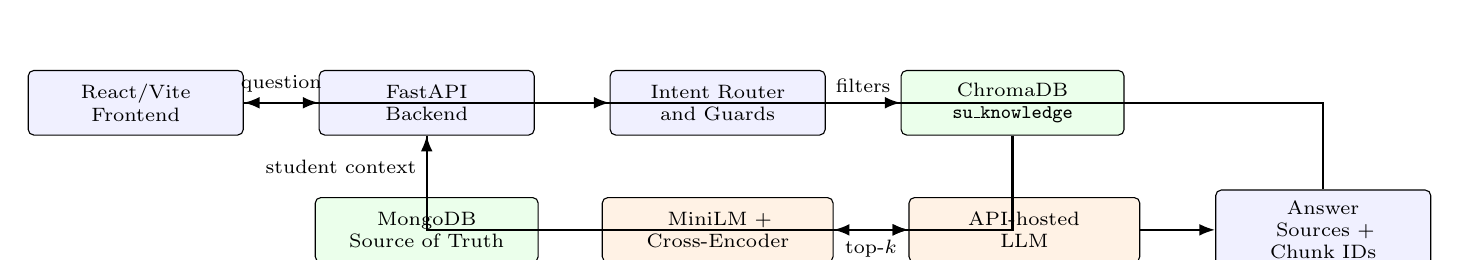
\begin{tikzpicture}[
  font=\scriptsize,
  node distance=0.78cm and 0.95cm,
  box/.style={draw, rounded corners=2pt, align=center, text width=2.45cm, minimum height=0.82cm, fill=blue!6, inner sep=4pt},
  store/.style={draw, rounded corners=2pt, align=center, text width=2.55cm, minimum height=0.82cm, fill=green!8, inner sep=4pt},
  model/.style={draw, rounded corners=2pt, align=center, text width=2.65cm, minimum height=0.82cm, fill=orange!10, inner sep=4pt},
  arrow/.style={-{Latex[length=2mm]}, thick}
]
\node[box] (ui) {React/Vite\\Frontend};
\node[box, right=of ui] (api) {FastAPI\\Backend};
\node[box, right=of api] (router) {Intent Router\\and Guards};
\node[store, below=of api] (mongo) {MongoDB\\Source of Truth};
\node[store, right=of router] (chroma) {ChromaDB\\\texttt{su\_knowledge}};
\node[model, below=of router] (embed) {MiniLM +\\Cross-Encoder};
\node[model, right=of embed] (llm) {API-hosted\\LLM};
\node[box, right=of llm] (answer) {Answer\\Sources + Chunk IDs};
\draw[arrow] (ui) -- node[above]{question} (api);
\draw[arrow] (api) -- (router);
\draw[arrow] (router) -- node[above]{filters} (chroma);
\draw[arrow] (chroma) |- (embed);
\draw[arrow] (embed) -- node[below]{top-$k$} (llm);
\draw[arrow] (mongo) -- node[left]{student context} (api);
\draw[arrow] (api) |- (llm);
\draw[arrow] (llm) -- (answer);
\draw[arrow] (answer) |- (ui);
\end{tikzpicture}
}
\caption{Runtime architecture of SU-GPT. The measured local configuration uses MongoDB via Docker and ChromaDB persistence; the storage contract is compatible with a later managed deployment.}
\label{fig:architecture}
\end{figure}


\subsection{Frontend and Backend}
The frontend is implemented with React and Vite. It contains the chat interface, authentication view, course-selection UI, and document-upload controls. The backend is implemented with FastAPI. The \texttt{/ask/} endpoint receives a question and optional username, resolves intent, retrieves or constructs context, loads user course history, builds the prompt, invokes the LLM, and returns the generated answer with sources.

The LLM provider is configurable. The measured local run used \texttt{LLM\_PROVIDER=mistral} with \texttt{mistral-small-latest}; the project also contains Groq/Llama configuration for deployments that use Groq-hosted Llama 3.3 70B. The report therefore describes the architecture as API-hosted LLM-ready rather than tying all measured results to one provider.

\subsection{MongoDB Source of Truth}
MongoDB stores structured application state, including users, course records, user-course selections, source documents, ingestion jobs, upload batches, reviews, exams, and embedding-cache metadata. In local experiments, MongoDB runs via Docker; the schema is compatible with a managed MongoDB Atlas deployment. ChromaDB is not the source of truth. It is a reproducible vector index that can be rebuilt from MongoDB source metadata and stored files.

\subsection{ChromaDB Vector Index}
ChromaDB stores retrieval-ready text, vector embeddings, metadata, and stable chunk identifiers in the \texttt{su\_knowledge} collection. The active local index contains 229{,}631 chunks. All indexed chunks in the current benchmark-relevant corpus use \texttt{documentType=course}; review and exam corpora are intentionally empty in this phase.

\begin{table}[H]
\centering
\caption{Principal system components in the current implementation.}
\label{tab:components}
\begin{tabular}{ll}
\toprule
Component & Technology / Current Role \\
\midrule
Frontend & React + Vite \\
Backend & FastAPI + Python \\
Operational database & MongoDB, local Docker in measured run; Atlas-ready schema \\
Vector database & ChromaDB, \texttt{su\_knowledge} collection \\
Embedding model & \texttt{sentence-transformers/all-MiniLM-L12-v2} \\
Reranker & \texttt{cross-encoder/ms-marco-MiniLM-L-6-v2} \\
Generator & API-hosted LLM; measured local run used Mistral \\
Evaluation outputs & JSONL/JSON/CSV under \texttt{outputs/} \\
\bottomrule
\end{tabular}
\end{table}

\section{Data and Preprocessing}
\subsection{Data Sources}
The benchmark-relevant data comes from JSONL course and curriculum records plus uploaded course-material sources. Table~\ref{tab:data-sources} lists the main structured sources.

\begin{table}[H]
\centering
\caption{Main data sources and roles.}
\label{tab:data-sources}
\begin{tabular}{p{0.43\linewidth}p{0.48\linewidth}}
\toprule
Path & Role \\
\midrule
\texttt{data/all\_coursepage\_info.jsonl} & Course titles, descriptions, credits, prerequisites, corequisites, source URLs. \\
\texttt{data/\{term\}/\{program\}.jsonl} & Program-term classification snapshots, SU credits, ECTS, engineering ECTS, basic-science ECTS. \\
\shortstack[l]{\texttt{data/degree\_requirements/}\\\texttt{CS.jsonl}} & Detailed BSCS requirements for curriculum term 202101. \\
\texttt{data/schedule/202502.jsonl} & Sections, CRNs, instructors, meeting times, rooms, and components. \\
\shortstack[l]{\texttt{data/graduation\_}\\\texttt{requirements.jsonl}} & General graduation requirement records. \\
\texttt{sources/Module*} & CS455/555 course-material documents used for lecture-content retrieval. \\
\bottomrule
\end{tabular}
\end{table}

\subsection{Ingestion}
\begin{figure}[H]
\centering
\resizebox{0.94\linewidth}{!}{%
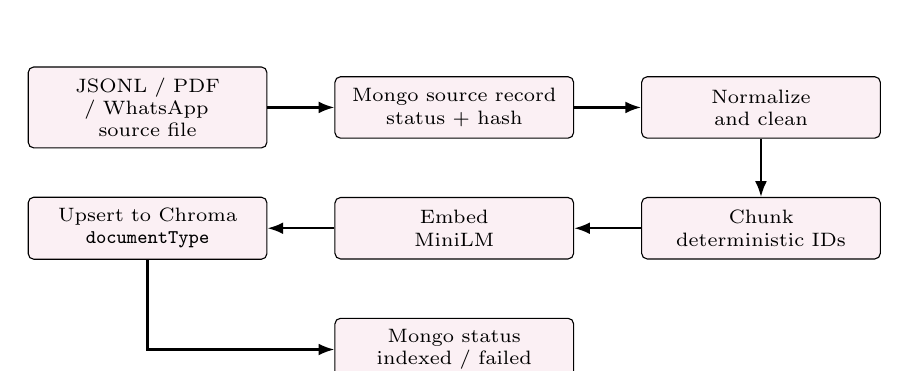
\begin{tikzpicture}[
  font=\scriptsize,
  node distance=0.74cm and 0.85cm,
  stage/.style={draw, rounded corners=2pt, align=center, text width=2.75cm, minimum height=0.78cm, fill=purple!6, inner sep=4pt},
  arrow/.style={-{Latex[length=2mm]}, thick}
]
\node[stage] (src) {JSONL / PDF / WhatsApp\\source file};
\node[stage, right=of src] (mongo) {Mongo source record\\status + hash};
\node[stage, right=of mongo] (norm) {Normalize\\and clean};
\node[stage, below=of norm] (chunk) {Chunk\\deterministic IDs};
\node[stage, left=of chunk] (embed) {Embed\\MiniLM};
\node[stage, left=of embed] (upsert) {Upsert to Chroma\\\texttt{documentType}};
\node[stage, below=of embed] (status) {Mongo status\\indexed / failed};
\draw[arrow] (src) -- (mongo);
\draw[arrow] (mongo) -- (norm);
\draw[arrow] (norm) -- (chunk);
\draw[arrow] (chunk) -- (embed);
\draw[arrow] (embed) -- (upsert);
\draw[arrow] (upsert) |- (status);
\end{tikzpicture}
}
\caption{Unified ingestion backbone. MongoDB stores durable source-of-truth metadata; ChromaDB is treated as a reproducible index.}
\label{fig:ingestion}
\end{figure}


Structured rows are converted into explanatory information cards. A course-catalog row becomes a short card with course code, title, credits, prerequisites, corequisites, description, and source URL. A schedule row becomes a card with term, CRN, instructor, meeting time, room, and component. Every chunk receives a deterministic ID with the shape:

\begin{center}
\texttt{sourceId:chunkIndex:contentHashPrefix}
\end{center}

The measured benchmark contains verified chunk IDs. For example:
\begin{center}
{\scriptsize\texttt{course:5a6a448569ef18c6d8137810:150:5f9083e5db8d5499}}
\end{center}
These stable IDs allow retrieval metrics to be computed at the chunk level.

\section{Question-Answering Pipeline}
\subsection{Intent Routing and Source Availability}
The system first predicts or resolves an intent. The current routes include graduation status, course recommendation, study plan, major selection, specialization, course detail, review, exam, and general fallback. When local evidence is available, the answer should be grounded in retrieved context. When local evidence is intentionally absent, as for review, exam, and syllabus-specific corpora in this phase, the system should state that it lacks a local source and provide cautious general guidance instead of pretending to have retrieved evidence. For example, a missing-review answer can advise the student to check course groups or email the instructor with a short background and question, while clearly marking that no local review archive was used.

\subsection{Retrieval and Generation}
The default final context size is $k=6$. Dense retrieval uses Chroma similarity search. Hybrid rerank combines BM25 and dense candidates, fuses them with RRF, and reranks with a cross-encoder. The final response includes both \texttt{sources} and \texttt{source\_chunk\_ids}.

\begin{figure}[H]
\centering
\resizebox{0.94\linewidth}{!}{%
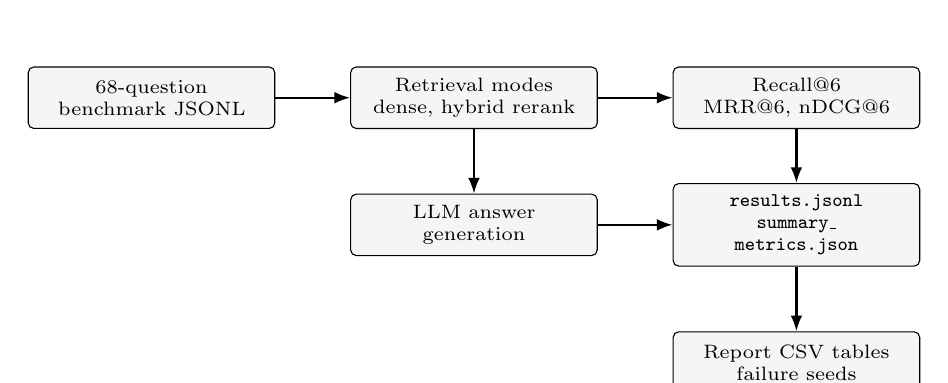
\begin{tikzpicture}[
  font=\scriptsize,
  node distance=0.82cm and 0.95cm,
  box/.style={draw, rounded corners=2pt, align=center, text width=2.85cm, minimum height=0.78cm, fill=gray!8, inner sep=4pt},
  arrow/.style={-{Latex[length=2mm]}, thick}
]
\node[box] (bench) {68-question\\benchmark JSONL};
\node[box, right=of bench] (modes) {Retrieval modes\\dense, hybrid rerank};
\node[box, right=of modes] (metrics) {Recall@6\\MRR@6, nDCG@6};
\node[box, below=of modes] (gen) {LLM answer\\generation};
\node[box, right=of gen] (outputs) {\texttt{results.jsonl}\\\texttt{summary\_}\\\texttt{metrics.json}};
\node[box, below=of outputs] (tables) {Report CSV tables\\failure seeds};
\draw[arrow] (bench) -- (modes);
\draw[arrow] (modes) -- (metrics);
\draw[arrow] (modes) -- (gen);
\draw[arrow] (metrics) -- (outputs);
\draw[arrow] (gen) -- (outputs);
\draw[arrow] (outputs) -- (tables);
\end{tikzpicture}
}
\caption{Evaluation pipeline implemented for the current measured pilot run. Full 68-question, six-mode execution is supported by the CLI but remains to be run before final numeric claims are frozen.}
\label{fig:evaluation-flow}
\end{figure}


\section{Evaluation Methodology}
\subsection{Benchmark}
The current benchmark file contains 68 grounded questions. Each JSONL row includes an ID, question, language, question type, expected intent, expected document type, answerability flag, reference answer, expected sources, expected chunk IDs, and notes. Every expected chunk ID was verified against the live \texttt{su\_knowledge} collection before evaluation.

\begin{table}[H]
\centering
\caption{Benchmark composition from \texttt{data/benchmark/questions.jsonl}.}
\label{tab:benchmark-composition}
\begin{tabular}{llr}
\toprule
Document type & Intent / answerability group & Count \\
\midrule
course & \texttt{ders\_ayrintisi}, answerable & 20 \\
course & \texttt{diger}, answerable & 20 \\
course & \texttt{diger}, unanswerable & 16 \\
course & \texttt{mezuniyet\_durumu}, answerable & 7 \\
exam & \texttt{exam}, unanswerable & 2 \\
review & \texttt{review}, unanswerable & 2 \\
course & \texttt{ders\_ayrintisi}, unanswerable & 1 \\
\midrule
Total & & 68 \\
\bottomrule
\end{tabular}
\end{table}

\subsection{Metrics}
Retrieval is measured with Recall@K, MRR@K, and nDCG@K. Chunk-level matching is used when \texttt{expected\_chunk\_ids} exist. If a row has no expected chunk IDs, the evaluator falls back to source-level matching using \texttt{expected\_sources}. For the measured pilot run, $K=6$ because the runner defaulted to \texttt{top\_k=6}.

\begin{align}
\mathrm{Recall@K} &= \frac{|\mathrm{Retrieved}_{1:K} \cap \mathrm{Gold}|}{|\mathrm{Gold}|},\\
\mathrm{MRR@K} &= \frac{1}{\mathrm{rank\ of\ first\ relevant\ hit}},\\
\mathrm{nDCG@K} &= \frac{\mathrm{DCG@K}}{\mathrm{IDCG@K}}.
\end{align}

\subsection{Measured Run}
The current measured run is stored under \texttt{outputs/evaluation\_runs/20260607\_231717}. It evaluated the first 10 benchmark questions with two modes: dense and hybrid rerank. LLM generation was enabled. This gives 20 result rows and 120 retrieved-chunk rows.

\todoresult{Before final submission, run the full benchmark with all six modes, or explicitly state that the project reports a pilot evaluation only. The CLI already supports this via \texttt{server/evaluation/run\_evaluation.py}.}

\section{Results}
\subsection{Retrieval Metrics}
\begin{figure}[H]
\centering
\resizebox{0.78\linewidth}{!}{%
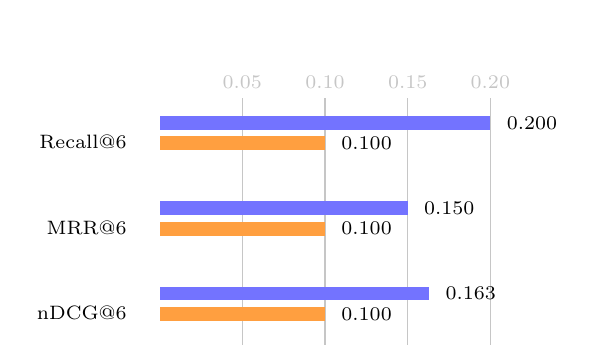
\begin{tikzpicture}[x=21cm,y=0.62cm,font=\scriptsize]
\foreach \x/\lab in {0.05/0.05,0.10/0.10,0.15/0.15,0.20/0.20}
  \draw[gray!45] (\x,0.58) -- (\x,5.85) node[above]{\lab};

\node[anchor=east] at (-0.014,4.95) {Recall@6};
\fill[blue!55] (0,5.20) rectangle (0.20,5.48);
\node[anchor=west] at (0.204,5.34) {0.200};
\fill[orange!75] (0,4.78) rectangle (0.10,5.06);
\node[anchor=west] at (0.104,4.92) {0.100};

\node[anchor=east] at (-0.014,3.20) {MRR@6};
\fill[blue!55] (0,3.45) rectangle (0.15,3.73);
\node[anchor=west] at (0.154,3.59) {0.150};
\fill[orange!75] (0,3.03) rectangle (0.10,3.31);
\node[anchor=west] at (0.104,3.17) {0.100};

\node[anchor=east] at (-0.014,1.45) {nDCG@6};
\fill[blue!55] (0,1.70) rectangle (0.163,1.98);
\node[anchor=west] at (0.167,1.84) {0.163};
\fill[orange!75] (0,1.28) rectangle (0.10,1.56);
\node[anchor=west] at (0.104,1.42) {0.100};
\end{tikzpicture}
}
\caption{Measured pilot retrieval metrics on the first 10 benchmark questions. Blue bars show dense retrieval; orange bars show hybrid rerank. The run used $k=6$ and generated LLM answers.}
\label{fig:retrieval-metrics}
\end{figure}


\begin{table}[H]
\centering
\caption{Measured pilot retrieval results on the first 10 questions, $K=6$.}
\label{tab:retrieval-results}
\begin{tabular}{lrrrrr}
\toprule
Mode & Rows & Recall@6 & MRR@6 & nDCG@6 & Chunk hit rate \\
\midrule
Dense & 10 & 0.200 & 0.150 & 0.163 & 0.200 \\
Hybrid rerank & 10 & 0.100 & 0.100 & 0.100 & 0.100 \\
\bottomrule
\end{tabular}
\end{table}

On this small pilot slice, dense retrieval outperformed hybrid rerank. This should not be interpreted as a universal conclusion, because the sample is only the first 10 benchmark rows and the hybrid path paid a substantial retrieval/reranking cost. The result is nevertheless useful: it shows that hybrid and rerank logic can fail if the right chunk is absent from the candidate set or if near-identical template rows dominate the fused ranking.

\subsection{Latency and Efficiency}
\begin{figure}[H]
\centering
\resizebox{0.78\linewidth}{!}{%
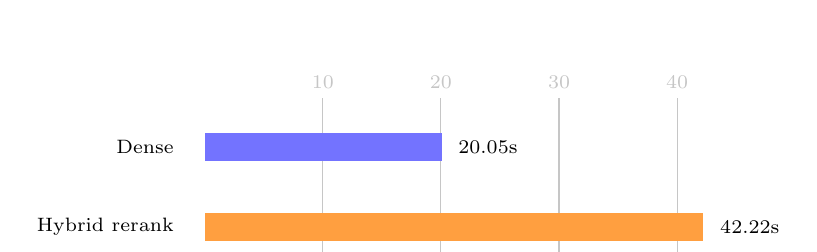
\begin{tikzpicture}[x=0.15cm,y=0.78cm,font=\scriptsize]
\foreach \x in {10,20,30,40}
  \draw[gray!45] (\x,0.48) -- (\x,3.15) node[above]{\x};

\node[anchor=east] at (-1.8,2.35) {Dense};
\fill[blue!55] (0,2.12) rectangle (20.05,2.58);
\node[anchor=west] at (20.65,2.35) {20.05s};

\node[anchor=east] at (-1.8,1.05) {Hybrid rerank};
\fill[orange!75] (0,0.82) rectangle (42.22,1.28);
\node[anchor=west] at (42.82,1.05) {42.22s};
\end{tikzpicture}
}
\caption{Mean end-to-end latency for the measured pilot run, including retrieval and generation. Blue indicates dense retrieval and orange indicates hybrid rerank. Hybrid rerank was slower primarily because retrieval and reranking dominate the runtime.}
\label{fig:latency}
\end{figure}


\begin{table}[H]
\centering
\caption{Measured pilot efficiency metrics. Values are averages across the 10 questions per mode.}
\label{tab:efficiency-results}
\begin{tabular}{lrrrr}
\toprule
Mode & Total latency & Retrieval & Rerank & Generation \\
\midrule
Dense & 20.05s & 18.36s & 0.00s & 1.69s \\
Hybrid rerank & 42.22s & 36.60s & 3.35s & 2.25s \\
\bottomrule
\end{tabular}
\end{table}

The primary bottleneck is retrieval over the large local Chroma/BM25 corpus, not LLM generation. A previous interactive \texttt{/ask/} optimization reduced common structured academic queries to below 10 seconds by bypassing broad vector search for intents that can be answered from structured catalog files. The benchmark runner, however, intentionally measures retrieval modes directly, so its latency exposes the raw retrieval cost.

\subsection{Answer Metrics}
\todoresult{Manual answer correctness, citation correctness, faithfulness, answer relevancy, and hallucination labels have not been filled. The generated \texttt{outputs/tables/answer\_metrics.csv} keeps these fields blank rather than fabricating scores. Fill them after a manual grading pass over \texttt{results.jsonl}.}

\section{Failure Analysis}
The Section 6 tooling currently contains two real seed failure cases in:
\begin{center}
{\scriptsize\texttt{outputs/failure\_analysis/failure\_cases.csv}}
\end{center}
Both are retrieval misses under hybrid rerank with $K=6$.

\begin{table}[H]
\centering
\caption{Seed failure cases from observed runs.}
\label{tab:failure-cases}
\begin{tabular}{p{0.12\linewidth}p{0.25\linewidth}p{0.20\linewidth}p{0.32\linewidth}}
\toprule
ID & Question type & Error type & Observed root cause \\
\midrule
q008 & CS412 schedule lookup & retrieval miss & The verified CS412 schedule chunk was absent from top-6; near-identical 202502 schedule chunks for other courses outranked the exact course row. \\
q020 & BERT position-embedding slide lookup & retrieval miss & The gold slide 17 chunk was very short; neighboring/richer chunks such as slide 16 ranked above the exact title-only slide. \\
\bottomrule
\end{tabular}
\end{table}

\subsection{Course-Code and Schedule Ambiguity}
Schedule records are highly template-like. A query mentioning \texttt{CS412} can retrieve other course sections from the same term because the surrounding text is nearly identical. Exact course-code extraction and normalized metadata filtering should run before dense/BM25 fusion for schedule questions.

\subsection{Short Chunk Weakness}
The q020 miss shows that short slide-title chunks can be under-ranked. A title such as ``Position Embeddings (Intuition)'' contains too little context compared with neighboring slides. A practical fix is to merge very short slide-title chunks with adjacent slide text or add title/slide-number boosts when a question asks about a specific slide.

\subsection{Missing Review, Exam, and Syllabus Sources}
The project currently has zero review chunks and zero exam chunks by design. The assistant must not claim retrieved review or exam evidence. The appropriate behavior is to say that the project is still under development for that source type, give cautious general guidance, and suggest checking official materials, student groups, or emailing the instructor. This policy should be evaluated separately from course-catalog retrieval.

\section{Ablations}
The Section 6 configuration file defines a future grid over chunk sizes, chunk overlaps, top-$k$ values, retrieval modes, and prompt strategies. Only a tiny quick ablation has been run so far: dense retrieval with top-$k=3$ over one benchmark question, which produced zero hit metrics and an average latency of 16.58 seconds. This is a smoke test of the ablation runner, not a scientific ablation result.

\todoresult{Run the full retrieval-only ablation grid after the final benchmark run. Prompt strategies \texttt{few\_shot} and \texttt{expert\_routed} should remain skipped until Section 4 prompt/router modules exist.}

\section{Limitations and Future Work}
The current system is not yet reliable as an official multi-program degree advisor. Detailed official degree requirements are available only for the CS/BSCS 202101 curriculum in the current structured file. User profiles need major, degree code, admission term, curriculum term, current term, minor codes, course status, transfer status, repeated-course handling, and withdrawal status.

Academic arithmetic should move out of the LLM and into a deterministic degree-audit module. The LLM should explain the computed result, not decide category allocation. Future degree-audit logic should apply equivalencies, choice pools, overflow rules, repeated-course handling, total SU credits, ECTS, engineering ECTS, basic-science ECTS, and GPA constraints.

Immediate retrieval improvements include:
\begin{itemize}
\setlength\itemsep{0.18em}
  \item normalize compact and spaced course identifiers at ingestion and query time;
  \item add exact course-code filters or boosts for schedule and catalog queries;
  \item enrich very short slide-title chunks with neighboring context;
  \item separate public curriculum sources from private student-specific degree evaluations;
  \item complete the full 68-question, six-mode benchmark run;
  \item manually grade answer correctness and citation correctness;
  \item expand unsupported review/exam/syllabus behavior tests so the assistant gives useful caveated advice without pretending to have local evidence.
\end{itemize}

\section{Reproducibility}
Backend setup:
\begin{verbatim}
cd server
python -m venv .venv
.venv/bin/pip install -r requirements.txt
docker compose up -d mongo
.venv/bin/python -m uvicorn main:app --host 127.0.0.1 --port 8000
\end{verbatim}

Frontend setup:
\begin{verbatim}
cd frontend
npm install
npm run dev
\end{verbatim}

Evaluation runner:
\begin{verbatim}
server/.venv/bin/python server/evaluation/run_evaluation.py \
  --modes dense hybrid_rerank --limit 10
\end{verbatim}

The reported pilot metrics were produced from \texttt{outputs/evaluation\_runs/20260607\_231717}. Report tables were generated under \texttt{outputs/tables/}. The current run used $K=6$.

\section{Ethical Considerations and AI Disclosure}
Academic advice can affect important student decisions. SU-GPT should not claim that a student can graduate unless the result uses the correct official curriculum and a complete student record. Answers must remain advisory and direct students to official Degree Evaluation and advisors for final confirmation.

Course histories and uploaded academic records are personal data. Future versions should enforce authentication, ownership filters, access control, and deletion policies. Private student documents must never be retrievable by another user.

Generative AI tools were used as development assistants for codebase analysis, debugging, evaluation tooling, documentation, and report drafting. The project members remain responsible for reviewing code, running experiments, checking source data, and validating reported results. Numerical values in this paper are copied from measured local output files and are not fabricated.

\section{Conclusion}
SU-GPT demonstrates a working retrieval-augmented academic advising application with a modern frontend, FastAPI backend, MongoDB source-of-truth model, ChromaDB vector index, deterministic ingestion, multiple retrieval modes, and a reproducible benchmark runner. The current measured pilot run is deliberately modest: 10 questions, two modes, and $K=6$. It still reveals important engineering facts. Dense retrieval reached Recall@6 of 0.20, while hybrid rerank reached 0.10 and incurred higher latency. The failures are mainly retrieval failures, not generation failures: the correct evidence often fails to reach the prompt.

The next step is not to make the model more fluent; it is to make retrieval more curriculum-aware. Exact course-code normalization, schedule-specific filters, short-chunk enrichment, deterministic degree auditing, and full benchmark execution are the most important steps before claiming official advising reliability.

\clearpage
\begin{thebibliography}{20}
\bibitem{lewis2020rag}
P. Lewis et al., ``Retrieval-Augmented Generation for Knowledge-Intensive NLP Tasks,'' \emph{NeurIPS}, 2020.

\bibitem{karpukhin2020dpr}
V. Karpukhin et al., ``Dense Passage Retrieval for Open-Domain Question Answering,'' \emph{EMNLP}, 2020.

\bibitem{guu2020realm}
K. Guu, K. Lee, Z. Tung, P. Pasupat, and M.-W. Chang, ``REALM: Retrieval-Augmented Language Model Pre-Training,'' \emph{ICML}, 2020.

\bibitem{izacard2021fid}
G. Izacard and E. Grave, ``Leveraging Passage Retrieval with Generative Models for Open Domain Question Answering,'' \emph{EACL}, 2021.

\bibitem{reimers2019sentencebert}
N. Reimers and I. Gurevych, ``Sentence-BERT: Sentence Embeddings using Siamese BERT-Networks,'' \emph{EMNLP-IJCNLP}, 2019.

\bibitem{nogueira2019passage}
R. Nogueira and K. Cho, ``Passage Re-ranking with BERT,'' arXiv:1901.04085, 2019.

\bibitem{robertson2009bm25}
S. Robertson and H. Zaragoza, ``The Probabilistic Relevance Framework: BM25 and Beyond,'' \emph{Foundations and Trends in Information Retrieval}, 2009.

\bibitem{cormack2009rrf}
G. V. Cormack, C. L. A. Clarke, and S. Buettcher, ``Reciprocal Rank Fusion Outperforms Condorcet and Individual Rank Learning Methods,'' \emph{SIGIR}, 2009.

\bibitem{khattab2020colbert}
O. Khattab and M. Zaharia, ``ColBERT: Efficient and Effective Passage Search via Contextualized Late Interaction over BERT,'' \emph{SIGIR}, 2020.

\bibitem{malkov2018hnsw}
Y. A. Malkov and D. A. Yashunin, ``Efficient and Robust Approximate Nearest Neighbor Search Using Hierarchical Navigable Small World Graphs,'' \emph{IEEE TPAMI}, 2018.

\bibitem{johnson2019faiss}
J. Johnson, M. Douze, and H. Jégou, ``Billion-Scale Similarity Search with GPUs,'' \emph{IEEE Transactions on Big Data}, 2019.

\bibitem{vaswani2017attention}
A. Vaswani et al., ``Attention Is All You Need,'' \emph{NeurIPS}, 2017.

\bibitem{devlin2019bert}
J. Devlin, M.-W. Chang, K. Lee, and K. Toutanova, ``BERT: Pre-training of Deep Bidirectional Transformers for Language Understanding,'' \emph{NAACL}, 2019.

\bibitem{wolf2020transformers}
T. Wolf et al., ``Transformers: State-of-the-Art Natural Language Processing,'' \emph{EMNLP: System Demonstrations}, 2020.

\bibitem{lin2021pretrained}
J. Lin, R. Nogueira, and A. Yates, ``Pretrained Transformers for Text Ranking: BERT and Beyond,'' \emph{Synthesis Lectures on Human Language Technologies}, 2021.

\bibitem{liu2024lost}
N. F. Liu et al., ``Lost in the Middle: How Language Models Use Long Contexts,'' \emph{TACL}, 2024.

\bibitem{openai2023gpt4}
OpenAI, ``GPT-4 Technical Report,'' arXiv:2303.08774, 2023.

\bibitem{langchain}
LangChain Documentation, \url{https://python.langchain.com/}.

\bibitem{chroma}
Chroma Documentation, \url{https://docs.trychroma.com/}.

\bibitem{mongodb}
MongoDB Atlas Documentation, \url{https://www.mongodb.com/docs/atlas/}.

\bibitem{sentence-transformers}
Sentence Transformers Documentation, \url{https://www.sbert.net/}.
\end{thebibliography}

\end{document}
